\documentclass[11pt]{extarticle}
\usepackage[tmargin=1in,bmargin=1in,lmargin=1in,rmargin=1in]{geometry}
\usepackage[utf8]{inputenc}
\usepackage{tikz}
\usepackage{graphicx}
\usepackage{float}
\usepackage{setspace}
\usepackage{tabularx}
\usepackage[utf8]{inputenc}
\usepackage{caption}
\usepackage{subcaption}
\usepackage{framed}
\usepackage{enumitem}
\usepackage{amsmath}
\usepackage{mathpazo}
\usepackage{ragged2e}
\usepackage{titlesec}
\usepackage{framed}
\usepackage{color}   %May be necessary if you want to color links
\usepackage{hyperref}
\usepackage{footnotebackref}
\usepackage{listings}
\usepackage{xcolor}
\usepackage{fancyhdr}
\usepackage{lastpage}
\usepackage{pgfplots}
\usepackage{lscape}
\usepackage{pdfpages}
\pgfplotsset{tick label style={font=\tiny}}

\hypersetup{
    colorlinks=true, %set true if you want colored links
    linktoc=section,     %set to all if you want both sections and subsections linked
    linkcolor=black,  %choose some color if you want links to stand out
}

\fancypagestyle{myheadings}
{
    \fancyhf{}
    \renewcommand{\footrulewidth}{0pt}
    \renewcommand{\headrulewidth}{0pt}
    \cfoot{Page \thepage\ of \pageref*{LastPage}}    
}

\fancypagestyle{plain}
{
    \fancyhf{}
    \chead{\small Delivery 05}
    \lhead{\small CS 353}
    \rhead{\small Spring 2022}
    % \renewcommand{\footrulewidth}{0.5pt}
    \renewcommand{\headrulewidth}{0.5pt}
    \cfoot{Page \thepage\ of \pageref*{LastPage}}    
}

\definecolor{mGreen}{rgb}{0,0.6,0}
\definecolor{mGray}{rgb}{0.5,0.5,0.5}
\definecolor{mPurple}{rgb}{0.58,0,0.82}
\definecolor{backgroundColour}{rgb}{0.95,0.95,0.92}

\lstdefinestyle{CStyle}{
    backgroundcolor=\color{backgroundColour},
    % backgroundcolor = \color{white},   
    commentstyle=\color{mGreen},
    keywordstyle=\color{magenta},
    numberstyle=\tiny\color{mGray},
    stringstyle=\color{mPurple},
    basicstyle=\footnotesize\bfseries\fontfamily{cmtt}\selectfont,
    breakatwhitespace=false,         
    breaklines=true,                 
    captionpos=b,                    
    keepspaces=true,                 
    numbers=left,                    
    numbersep=5pt,                  
    showspaces=false,                
    showstringspaces=false,
    showtabs=false,                  
    tabsize=2,
    frame = single,
    language=C
}

\title{\textbf{Project Delivery 03}}
\author{Aliza Rafique (05986); Asad Tariq (05439); Fahad Shaikh (05452); Faiz Haseeb (06224)}
\date{$8^{th}$ March 2022}


% Set formats for each heading level
\titleformat*{\section}{\Large\bfseries\fontfamily{phv}\selectfont}
\titleformat*{\subsection}{\large\bfseries\fontfamily{phv}\selectfont}
\titleformat*{\subsubsection}{\itshape\subsubsectionfont}

\providecommand\phantomsection{}

\doublespacing
\pgfplotsset{compat=1.18}
\begin{document}
\begin{titlepage}
\thispagestyle{empty}
\begin{center}

\includegraphics[scale=0.40]{Figures/HU-LOGO--01.jpg}
\line(1,0){400}\\
[2mm]
\fontfamily{phv}\selectfont
\textbf{Project Proposal}\\
\line(2,0){250}\\
[0.5cm]
Submitted By\\
Aliza Rafique (05986)\\
Asad Tariq (05439)\\
Fahad Shaikh (05452)\\
%Nom 2 (NI 2) \\ %À enlever le commentaire si jamais vous êtes plusieurs
[1.5cm]
CS353\\
Software Engineering\\ 
[1.0cm]
Section\\
L1\\
[1.0cm]
Instructor\\
Mohsin Nagaria\\
[1.5cm]
From the department of Computer Science\\
Dhanani School of Science and Engineering\\
Habib University\\
3$^{rd}$ February, 2022
\end{center} 
\end{titlepage}
\newpage
\thispagestyle{empty}
\tableofcontents
\newpage
\pagestyle{plain}

\section{Wireframes}
\justify
The following wireframes have been developed in accordance to the user stories of our application.

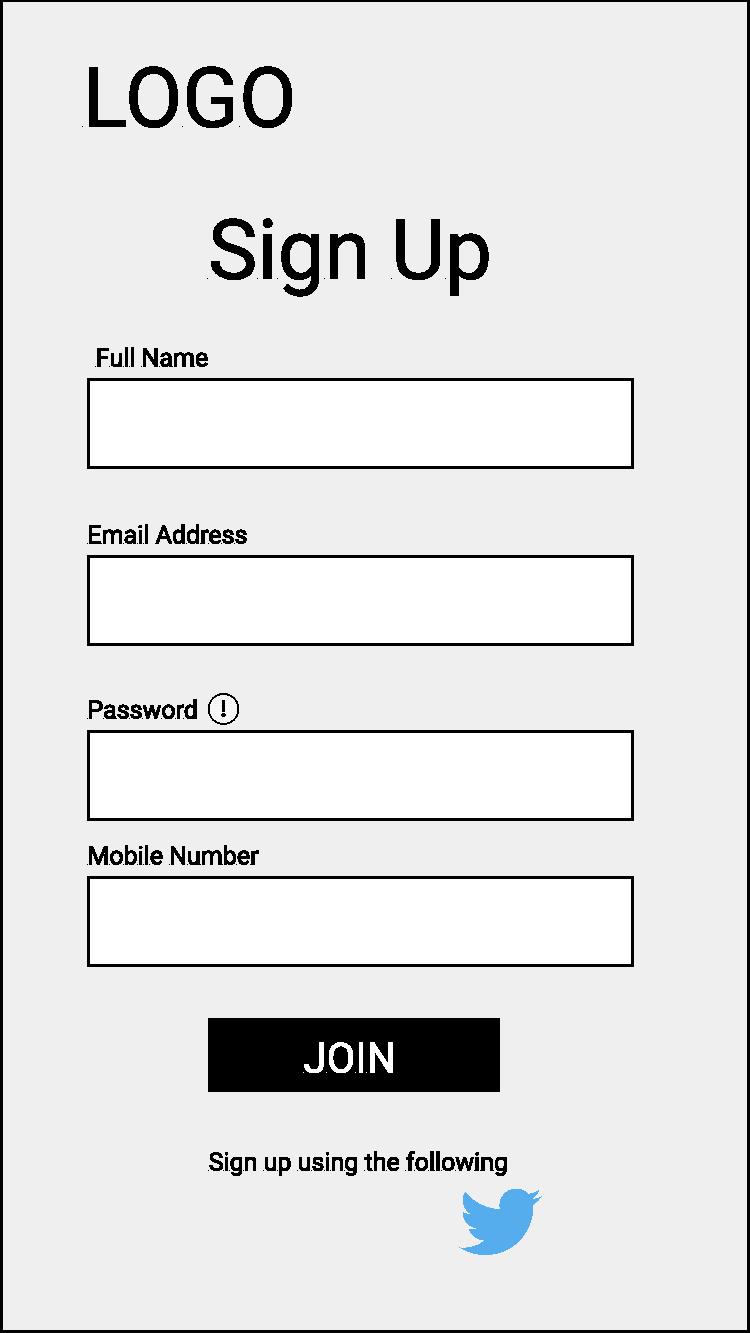
\includepdf[pages=-]{Wireframes.pdf}

\newpage
\section{User Stories}
\justify
The user stories of Meri Raye, that can be found on \href{https://trello.com/b/I4bgtgMu/software-engineering-project}{Trello} are as follows:

\begin{center}
    \begin{figure}[H]
        \centering
        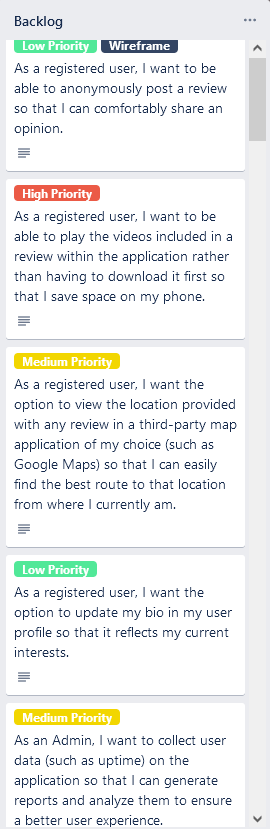
\includegraphics[width=2.4in]{Figures/user_stories_1.png}
        \caption{User stories of Meri Raye (set 1).}
    \end{figure}
\end{center}

\begin{center}
    \begin{figure}[H]
        \centering
        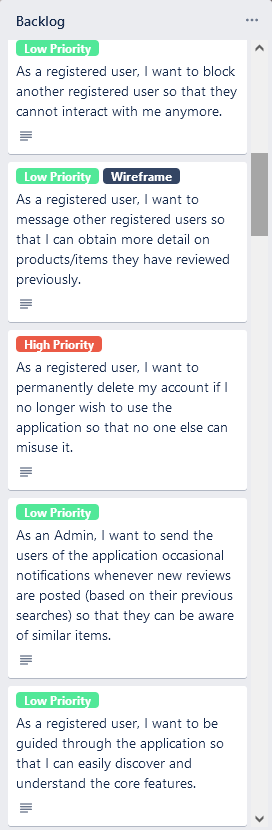
\includegraphics[width=2.4in]{Figures/user_stories_2.png}
        \caption{User stories of Meri Raye (set 2).}
    \end{figure}
\end{center}

\begin{center}
    \begin{figure}[H]
        \centering
        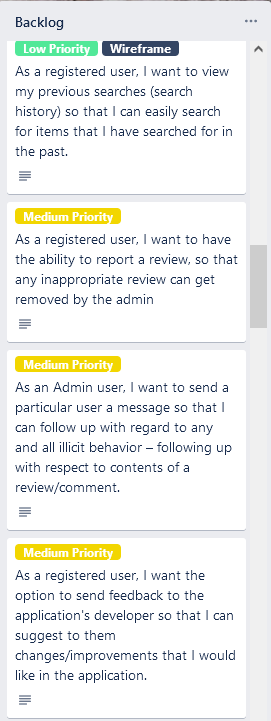
\includegraphics[width=2.4in]{Figures/user_stories_3.png}
        \caption{User stories of Meri Raye (set 3).}
    \end{figure}
\end{center}

\begin{center}
    \begin{figure}[H]
        \centering
        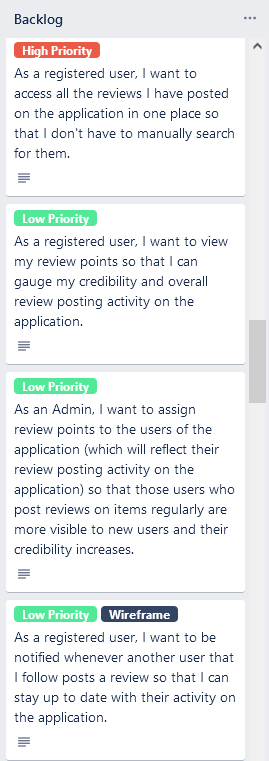
\includegraphics[width=2.4in]{Figures/user_stories_4.png}
        \caption{User stories of Meri Raye (set 4).}
    \end{figure}
\end{center}

\begin{center}
    \begin{figure}[H]
        \centering
        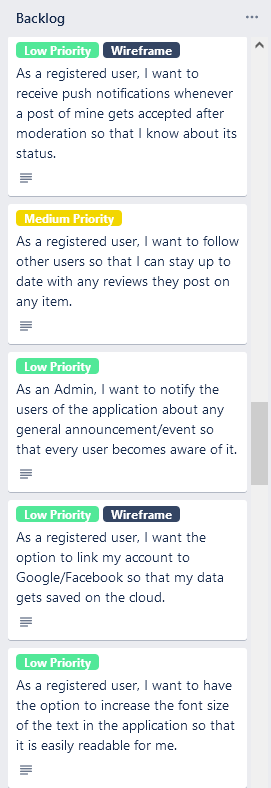
\includegraphics[width=2.4in]{Figures/user_stories_5.png}
        \caption{User stories of Meri Raye (set 5).}
    \end{figure}
\end{center}

\begin{center}
    \begin{figure}[H]
        \centering
        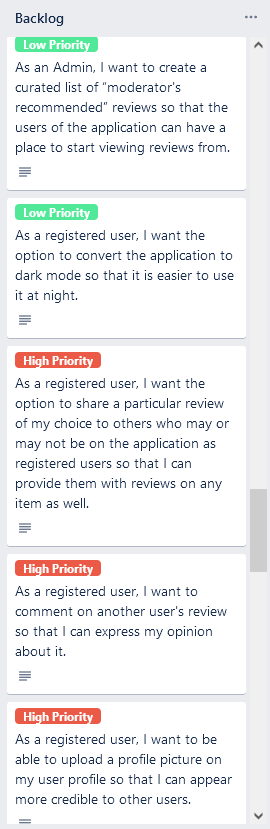
\includegraphics[width=2.4in]{Figures/user_stories_6.png}
        \caption{User stories of Meri Raye (set 6).}
    \end{figure}
\end{center}

\begin{center}
    \begin{figure}[H]
        \centering
        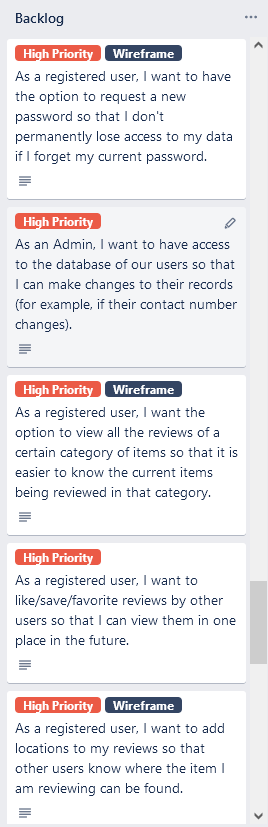
\includegraphics[width=2.4in]{Figures/user_stories_7.png}
        \caption{User stories of Meri Raye (set 7).}
    \end{figure}
\end{center}

\begin{center}
    \begin{figure}[H]
        \centering
        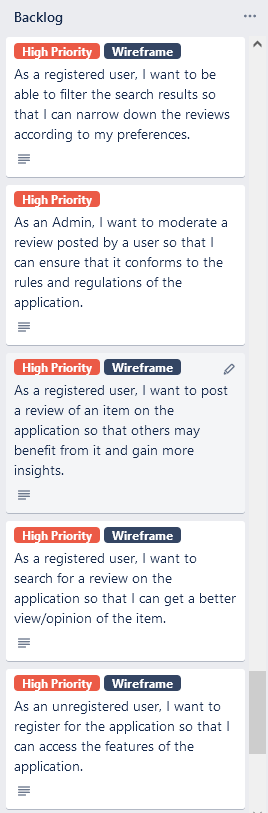
\includegraphics[width=2.4in]{Figures/user_stories_8.png}
        \caption{User stories of Meri Raye (set 8).}
    \end{figure}
\end{center}

\begin{center}
    \begin{figure}[H]
        \centering
        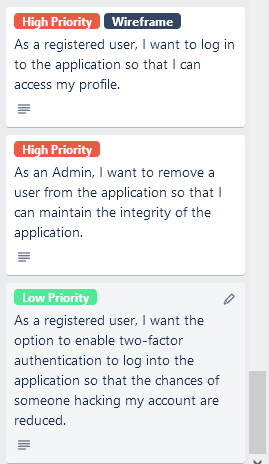
\includegraphics[width=2.4in]{Figures/user_stories_9.png}
        \caption{User stories of Meri Raye (set 9).}
    \end{figure}
\end{center}

\end{document}
